\documentclass[emulatestandardclasses]{scrartcl}
\usepackage{graphicx}
\usepackage{color}
\usepackage[ngerman]{babel}
\usepackage{hyperref}
\usepackage{fullpage}
\usepackage{calc} 
\usepackage{enumitem}
\usepackage{titlesec}
\newcommand{\todo}[1]{\textcolor{red}{TODO: #1}\PackageWarning{TODO:}{#1!}}
\date{\vspace{-3ex}}
\begin{document}

\title{
	\includegraphics*[width=0.75\textwidth]{ErstesSem/images/hu_logo.png}\\
	\vspace{24pt}
	Aristoteles\\Nikomachische Ethik}
\subtitle{VEV SS 17\\
          Dr. Philipp Br"ullmann\\
          Philosophische Fakult"at I \\ 
          Humboldt Universit"at zu Berlin}
\author{Lennard Wolf\\
        \small{\href{mailto:lennard.wolf@student.hu-berlin.de}{lennard.wolf@student.hu-berlin.de}}}
\maketitle
\begin{abstract}

Die Nikomachische Ethik des Aristoteles ist eine der interessantesten, einflussreichsten und meistdiskutierten Schriften zur praktischen Philosophie. Sie behandelt eine Vielzahl wichtiger Themen (wie etwa das gute Leben, Tugend, Verantwortung, Gerechtigkeit, Freundschaft, Willensschw"ache, Lust und Erziehung) und entwirft eine Konzeption der Ethik, die systematisch ernstzunehmen ist. Wer sich f"ur praktische Philosophie interessiert, sollte die Nikomachische Ethik kennen. In unserer Vorlesung werden wir uns (a) einen "uberblick "uber die zentralen Thesen und Argumente der Schrift verschaffen und dabei (b) einige Interpretationsprobleme und Forschungskontroversen kennenlernen. Außerdem werden wir (c) versuchen, die Nikomachische Ethik in ihren Kontext, d.h. den Kontext der antiken Ethik und der Aristotelischen Philosophie, einzuordnen und nicht zuletzt (d) immer wieder die Frage stellen, wie sich der Ansatz des Aristoteles zu anderen Ans"atzen in der normativen Ethik verh"alt.
\end{abstract}
\newpage

\tableofcontents
\listoffigures
\newpage


\section{Die Frage nach dem Gl"uck [I 1-5]\\(25.04.17)}

\subsection{Zusammenfassung erste Sitzung}

\begin{itemize}
  \item Unterscheidung Esoterisch/Exoterisch : Ver"offentlicht/Vorlesungen
  \item "`Gl"uck"': objektiv, kontingent
  \item "`Tugend"': technische Definition
  \item Ziel: Tugendhaft zu \emph{werden}, nicht blo"s Theorie kennen
  \item Enger Zusammenhang zwischen Tugend und Gl"uck
  \item Ethik hat hier nichts mit Moral zu tun
\end{itemize}

\noindent \textbf{Ziel der Sitzung:} Wie ist die Frage nach dem Gl"uck formuliert/wie ist das Problem beschrieben?

\subsection{\emph{eudaimonia}}

\begin{description}[leftmargin=!,labelwidth=\widthof{\bfseries Frage nach dem Gl"uck}]
  \item[Frage nach dem Gl"uck] Welches ist das beste Leben, das man f"uhren kann?
\end{description}


\subsection{Die Herausforderung des Amoralisten}

\begin{itemize}
  \item Frage nach dem guten Leben kam schon in Platons fr"uhen Dialogen vor (Sokrates)
  \item Sokrates versucht zu zeigen, dass der Gerechte ein besseres Leben hat als der Ungerechte (es ist f"ur \emph{ihn} besser, gerecht zu sein).
  \item Problem: intuitiv ist ungerecht sein doch von Vorteil f"ur einen
  \item Hirte Gyges (\emph{Politeia}): Ring kann unsichtbar machen, Hirte findet und kann heimlich Unrecht tun. "`W"urden wir das nicht auch alle machen?"'
  \item Herausforderung des Amoralisten: Warum sollen wir dann "uberhaupt gerecht sein?
  \item Genauer: einziger Vorteil eines gerechten Lebens ist Sicherheit vor Strafe
  \item Antwort von Sokrates: Gerechtigkeit ist ein bestimmter Zustand der Seele. Der Ungerechte schadet seiner Seele, er ist quasi \emph{krank}. (Unordnung in der Seele, die Teile der Seele tun nicht das wof"ur sie da sind)
\end{itemize}

\subsection{Aristoteles und der Amoralist}

\begin{itemize}
  \item Aufgabe: Zeigen, dass auch konsequent eigeninteressierte Menschen einen Grund haben, gerecht zu sein
  \item Aristoteles wendet sich nicht an den Amoralisten
  \item Eignet sich nicht f"ur Menschen, die sich nicht von ihren Leidenschaften bestimmen lassen, sowie sittenhaft und gut erzogen sind ($\rightarrow$ gemeinsame Grundlage)
  \item $\rightarrow$ was hei"st das f"ur die Moralpsychologie/das Begr"undungsprojekt?
\end{itemize}

\subsection{Die Frage nach dem Gl"uck}

\subsubsection{Das Anerkannte und das Umstrittene [I 2-3]}

\begin{itemize}
  \item Aristoteles fragt sich: Wor"uber besteht Einigkeit/Uneinigkeit?
  \item \textbf{Uneinigkeit}: Was ist das Gl"uck? | Vielfalt und Relativit"at der Antworten | Lebensformen... Lust (Menge): sklavenartig; Ehre (Politiker): abh"angig von anderen; Gutheit: w"are mit Unt"atigkeit vereinbar; Betrachtung (theoria): ???; Gelderwerb: Mittel zum Zweck
  \item \textbf{Einigkeit}: \emph{Das Gl"uck ist das h"ochste durch Handeln erreichbaren G"uter} (gut leben, handeln; sich wohl befinden)
  \item Diese Unterscheidung ist Grundlage f"ur Frage: Was ist das h"ochste Gut?
\end{itemize}

\subsubsection{G"uter und Ziele [I 1]}

\begin{itemize}
  \item Kede Kunst, Lehre, Handlung und Entschluss scheint irgendein Gut zu erstreben.
  \item G"uter sind Ziele; Das h"ochste Gut ist ein oberstes Ziel [I 1]
  \item Wenn $a$ das Ziel der T"atigkeit $b$ ist, dann ist $a$ "`besser"' (ein h"oheres Gut) als $b$. | Wenn $a$ ein Ziel ist, das wir umwillen eines h"ohren Ziels $b$ ist, dann ist $b$ "`besser"' (ein h"oheres Gut) als $a$.  | (G"uter k"onnen verglichen werden)
  \item H"ochstes Gut: Etwas das wir immer um seiner selbst willen und nie um einer anderen Sache willen erstreben und um dessentwillen wir alles andere erstreben
  \item Die \emph{eudaimonia} ist solch ein h"ochstes Gut
\end{itemize}

\subsubsection{Es gibt keine Idee des Guten [I 4]}

\begin{itemize}
  \item Begriff des h"ochsten Guts in Verkn"upfung mit Platons Ideenlehre: Gegenstand der \emph{gut} im "`h"ochsten Ma"se"' aufweist
  \item $\rightarrow$ Gradueller Unterschied (im Kontrast zu [I 1])
  \item Aristoteles weist diesen Ansatz zur"uck, da G"uter zu verschieden sind; Kennen des abstrakten Guten hilft nichts f"ur den Erwerb der einzelnen, konkreten G"uter
  \item $\rightarrow$ \emph{Nicht hintergehbare Verschiedenheit der G"uter}. Die Ethik muss dieser Verschiedenheit gerecht werden.
\end{itemize}

\subsubsection{Die drei Kriterien [I 5]}

\noindent \textbf{Kriterien die die eudaimonia als h"ochstes Gut auszeichnen:}

\begin{enumerate}
  \item Wir w"ahlen alles um des guten Lebens willen, aber niemals das gute Leben um einer anderen Sache willen.
  \item Die \emph{eudaimonia} ist "`autark"', d.h. wenn wir sie besitzen, dann bed"urfen wir keiner weiteren Dinge (betrifft auch andere Menschen).
  \item Die \emph{eudaimonia} l"asst sich nicht durch die Hinzuf"ugung weiterer G"uter verbessern.
\end{enumerate}

\noindent $\rightarrow$ Vorrauss"atzungen f"ur [I 6 ff.] eine eigene Bestimmung des Gl"ucks zu entwickeln

\subsection{Begriffe}

\begin{description}[leftmargin=!,labelwidth=\widthof{\bfseries \emph{eudaemonia}}]
  \item[\emph{eudaimonia}] \emph{Nicht}: Gl"ucksgef"uhl, oder Zufallsgl"uck | \emph{Sondern}: Ein insgesamt gelungenes Leben | W"ortlich: Unter "`gutem daimon"', unter einem guten Stern stehen (auch: \emph{Gl"uckseligkeit})
  \item[\emph{ergon}] Eigent"umliche Leistung | Ziel (Ergebnis -- muss nicht positiv sein!) einer T"atigkeit (\emph{techne}) | Um zu erkl"aren, was ein bestimmtes \emph{technite} ist, kommt man nicht umhin sein jeweiliges \emph{ergon} zu benennen
  \item[\emph{energeia}] Aktualit"at
  \item[\emph{dynamis}] M"oglichkeit/Potenzial
\end{description}

\subsection{Tutorium}

Wir verwenden die griechischen Ausdr"ucke


\section{Bestimmung des Gl"ucks [I 6-12]\\(02.05.17)}

\subsection{Das \emph{ergon} Argument [I 6]}

\subsubsection{Die Argumentstruktur}

\begin{description}[leftmargin=!,labelwidth=\widthof{\bfseries P3}]
  \item[P1] F"ur alle Gegenst"ande, die ein \emph{ergon} besitzen, liegt das \emph{agathon} und das \emph{eu} im \emph{ergon.}
  \item[P2] Der Mensch besitzt ein \emph{ergon}.
  \item[P3] Das \emph{ergon} des Menschen besteht in der T"atigkeit der Seele entsprechend der Vernunft. (Weil die Vernunft sein \emph{idios} ist)
  \item[K] Das Gute f"ur den Menschen liegt in der T"atigkeit der Seele entsprechend der Vernunft.
\end{description}

\subsubsection{Probleme mit dem Arguemnt}

\begin{itemize}
  \item Debatten "uber starke/schwache Lesart von \textbf{P1}
  \item Hat \textbf{P2} eine Begr"undung? Plausibel?
  \item Beruht das Argument auf einem "Aquivokationsfehlschluss? (Gut mit mehreren Bedeutungen?)
  \item Beruht das Argument auf einem problematischem Essentialismus? (Warum sollte es ein "`Wesen"' des Menschen geben? Warum sollte dieses normative Konsequenzen haben? | Moral basierend auf essentialistischen Pr"amissen ist schwierig)
  \item Ist das \emph{ergon} des Menschen richtig bestimmt? (Es gibt andere T"atigkeiten und F"ahigkeiten zu geben, die den Menschen vor anderen Lebewesen auszeichnen.)
\end{itemize}

\subsubsection{Eine deflation"are Lesart}

\begin{itemize}
  \item PLS COPY FROM FILE
\end{itemize}


\subsection{Vergleich mit den bestehenden Meinungen [I 8-12]}

\subsubsection{"Ubereinstimmung und Modifikation [I 8-9]}

\begin{itemize}
  \item Sein Vorschlag sollte "ubereinstimmen mit der gr"o"seren Menge der existierenden Meinungen
  \item Sie \textbf{stimmt "uberein} mit...
  \item PLS CPY
  \item "Au"sere Umst"ande k"onnen entweder $(a)$ Werkzeuge, oder $(b)$ Tr"ubung des Gl"ucks bedeuten. (Doch wie damit umgegangen werden soll steht im n"achsten Abschnitt.)
\end{itemize}

\subsubsection{Das Problem der "au"seren Ungl"ucksf"alle [I 10-11]}

\begin{itemize}
  \item PLS CPY
\end{itemize}

\subsection{Begriffe}

\begin{description}[leftmargin=!,labelwidth=\widthof{\bfseries \emph{makarios}}]
  \item[\emph{agathon}] Das Gute
  \item[\emph{eu}] Das "`auf gute Weise"' (Adverb von \emph{agathon})
  \item[\emph{psych\={e}}] Seele
  \item[\emph{idios}] Das einem Ding eigent"umliche
  \item[\emph{aret\={e}}] Tugend, Gutheit (noch nicht gekl"art)
  \item[\emph{makarios}] Seelig
  \item[\emph{athlios}] Elendig
\end{description}


\subsection{Tutorium}

\begin{description}[leftmargin=!,labelwidth=\widthof{\bfseries P3}]
  \item[P1] Ein "`abschlie"sendes Ziel"' (\emph{teleios}) ist ein solches, das niemals zum Zwecke eines anderen Zieles verfolgt wird.
  \item[P2] Das Gl"uck ist ein Ziel menschlichen Handelns (\emph{praxis}), das niemals zum Zwecke eines anderen Zieles verfolgt wird.
  \item[P3] Es gibt nur ein "`abschlie"sendes Ziel"' (\emph{teleios}) menschlichen Handelns (\emph{praxis}).
  \item[K] Das Gl"uck ist das "`abschlie"sende Ziel"' (\emph{teleios}) menschlichen Handelns (\emph{praxis}).
\end{description}


\section{Zwei Arten des Gl"ucks? [I 13; X 6-9]\\(09.05.17)}

\subsection{Lekt"urenotizen}

\noindent \textbf{[I 13]} Gutheit (\emph{aret\={e}}) = \emph{menschliche} Gutheit $\rightarrow$ Seele hat vernunftlosen (vegetativen) und vern"unftigen Bestandteil $\rightarrow$ Gutheit des vernunftlosen Bestandteils ist allen Tieren gleich und somit nicht relevant f"ur die \emph{menschliche} Gutheit $\rightarrow$ Es gibt in der Seele etwas das gegen die Vernunft wirkt (wie der Gegenmuskel) $\rightarrow$ Beide Bestandteile der Seele sind derart zweiteilig $\rightarrow$ Entsprechend wird die Gutheit auch zweigeteilt, und zwar in Tugenden des \emph{Denkens} und Tugenden des \emph{Charakters}\newline

\noindent \textbf{[X 6]} Gl"uck (\emph{eudaemonia}) ist keine Disposition (sonst k"onnte der Gute auch immerzu schlafen) $\rightarrow$ Handlungen der Gutheit: "uber diese hinaus sucht man nichts $\rightarrow$ Aber dies scheint auch f"ur Vergn"ugung zu gelten, und diese allein kann nicht gut sein, da f"ur die anderes vernachl"assigt wird (K"orper, Arbeit) $\rightarrow$ Das vernachl"assigte muss wieder erarbeitet werden und so m"ussen daraufhin Dinge getan werden, die nicht nur mit dem Gl"uck zum Ziele unternommen werden $\rightarrow$ Vergn"ugung ist also nicht Ziel, sondern lediglich ein Mittel daf"ur, Kraft f"ur gute T"atigkeiten zu sammeln \newline

\noindent \textbf{[X 7]} Betrachtung ist die h"ochste T"atigkeit, da ihr Gegenstand die h"ochsten Dinge sind, sie die kontinuierlichste ist, sie ernsthaft ist und ihr Weisheit (\emph{sophia}) beigemischt ist, welche die h"ochste Lust ist. Zudem ist sie autark und wird um ihrer selbst willen geliebt. | Die Betrachtung kann aber nicht die vollkommen einzige Bet"atigung sein, zudem h"atte dies etwas g"ottliches, un\emph{menschliches} -- keine menschliche Bet"atigung ist vollst"andig. Trotzdem ist es die "`gl"uckseligste"' aller T"atigkeiten.\newline

\noindent \textbf{[X 8]} Sekund"are Form des Gl"ucks wird erlangt durch guten Charakter, ausgedr"uckt durch gute Bet"atigung (\emph{energeia}): gerechtes, tapferes, angemessenes, kluges, richtiges Handeln. Solche Tugend ist aber getrennt von der Tugend des intuitiven Denkens (\emph{nous}, siehe [X 7]), welche die prim"are Form des Gl"ucks ist. Jede gute \emph{energeia} hat bestimmte Vorraussetzungen, so braucht der Tapfere einen starken K"orper usw. -- die Betrachtung aber hat keine/wenige Vorraussetzung. Die vollkommene Tugend liegt zugleich im Vorsatz und der damit verbundenen Handlung selbst. | Dass die Betrachtung die prim"are Form des Gl"ucks ist zeigt sich auch darin, dass die G"otter nicht handeln wie die Menschen (der Gedanke allein ist l"acherlich), aber ja insgesamt gl"uckselig sind, und somit wohl allein der Betrachtung fr"ohnen m"ussen.\newline

\noindent \textbf{[X 9]} Das gl"uckselige Leben bedarf bestimmter Umst"ande (genug zu essen usw.), doch nie im "Uberma"s: "`Auch mit bescheidenen Mitteln kann man n"amlich in Aus"ubung der Tugend handeln"', es gilt sich prim"ar im Sinn der Tugend zu bet"atigen. So brauch man, um den Gl"ucklichen zu finden, nicht nur bei den Reichen und M"achtigen suchen. Ob alles Gesagte zum Gl"uck wirklich wahr ist, l"asst sich nur durch Taten nachpr"ufen. | Die G"otter erfreuen sich an dem ihnen "ahnlichen, also dem Betrachtendem, dem Weisen. Dieser ist der gl"ucklichste und von den G"ottern am meisten geliebt.

\subsection{fgh [I 13]}

\begin{itemize}
  \item 
\end{itemize}

\subsection{Begriffe}

\begin{description}[leftmargin=!,labelwidth=\widthof{\bfseries \emph{eudaemonia}}]
  \item[\emph{agathon}] Das Gute
\end{description}

\subsection{Tutorium}



\newpage
\section{"Uber den Professor}
Prof. Mustermann ist..


%\begin{figure}[h]
%	\centering
%	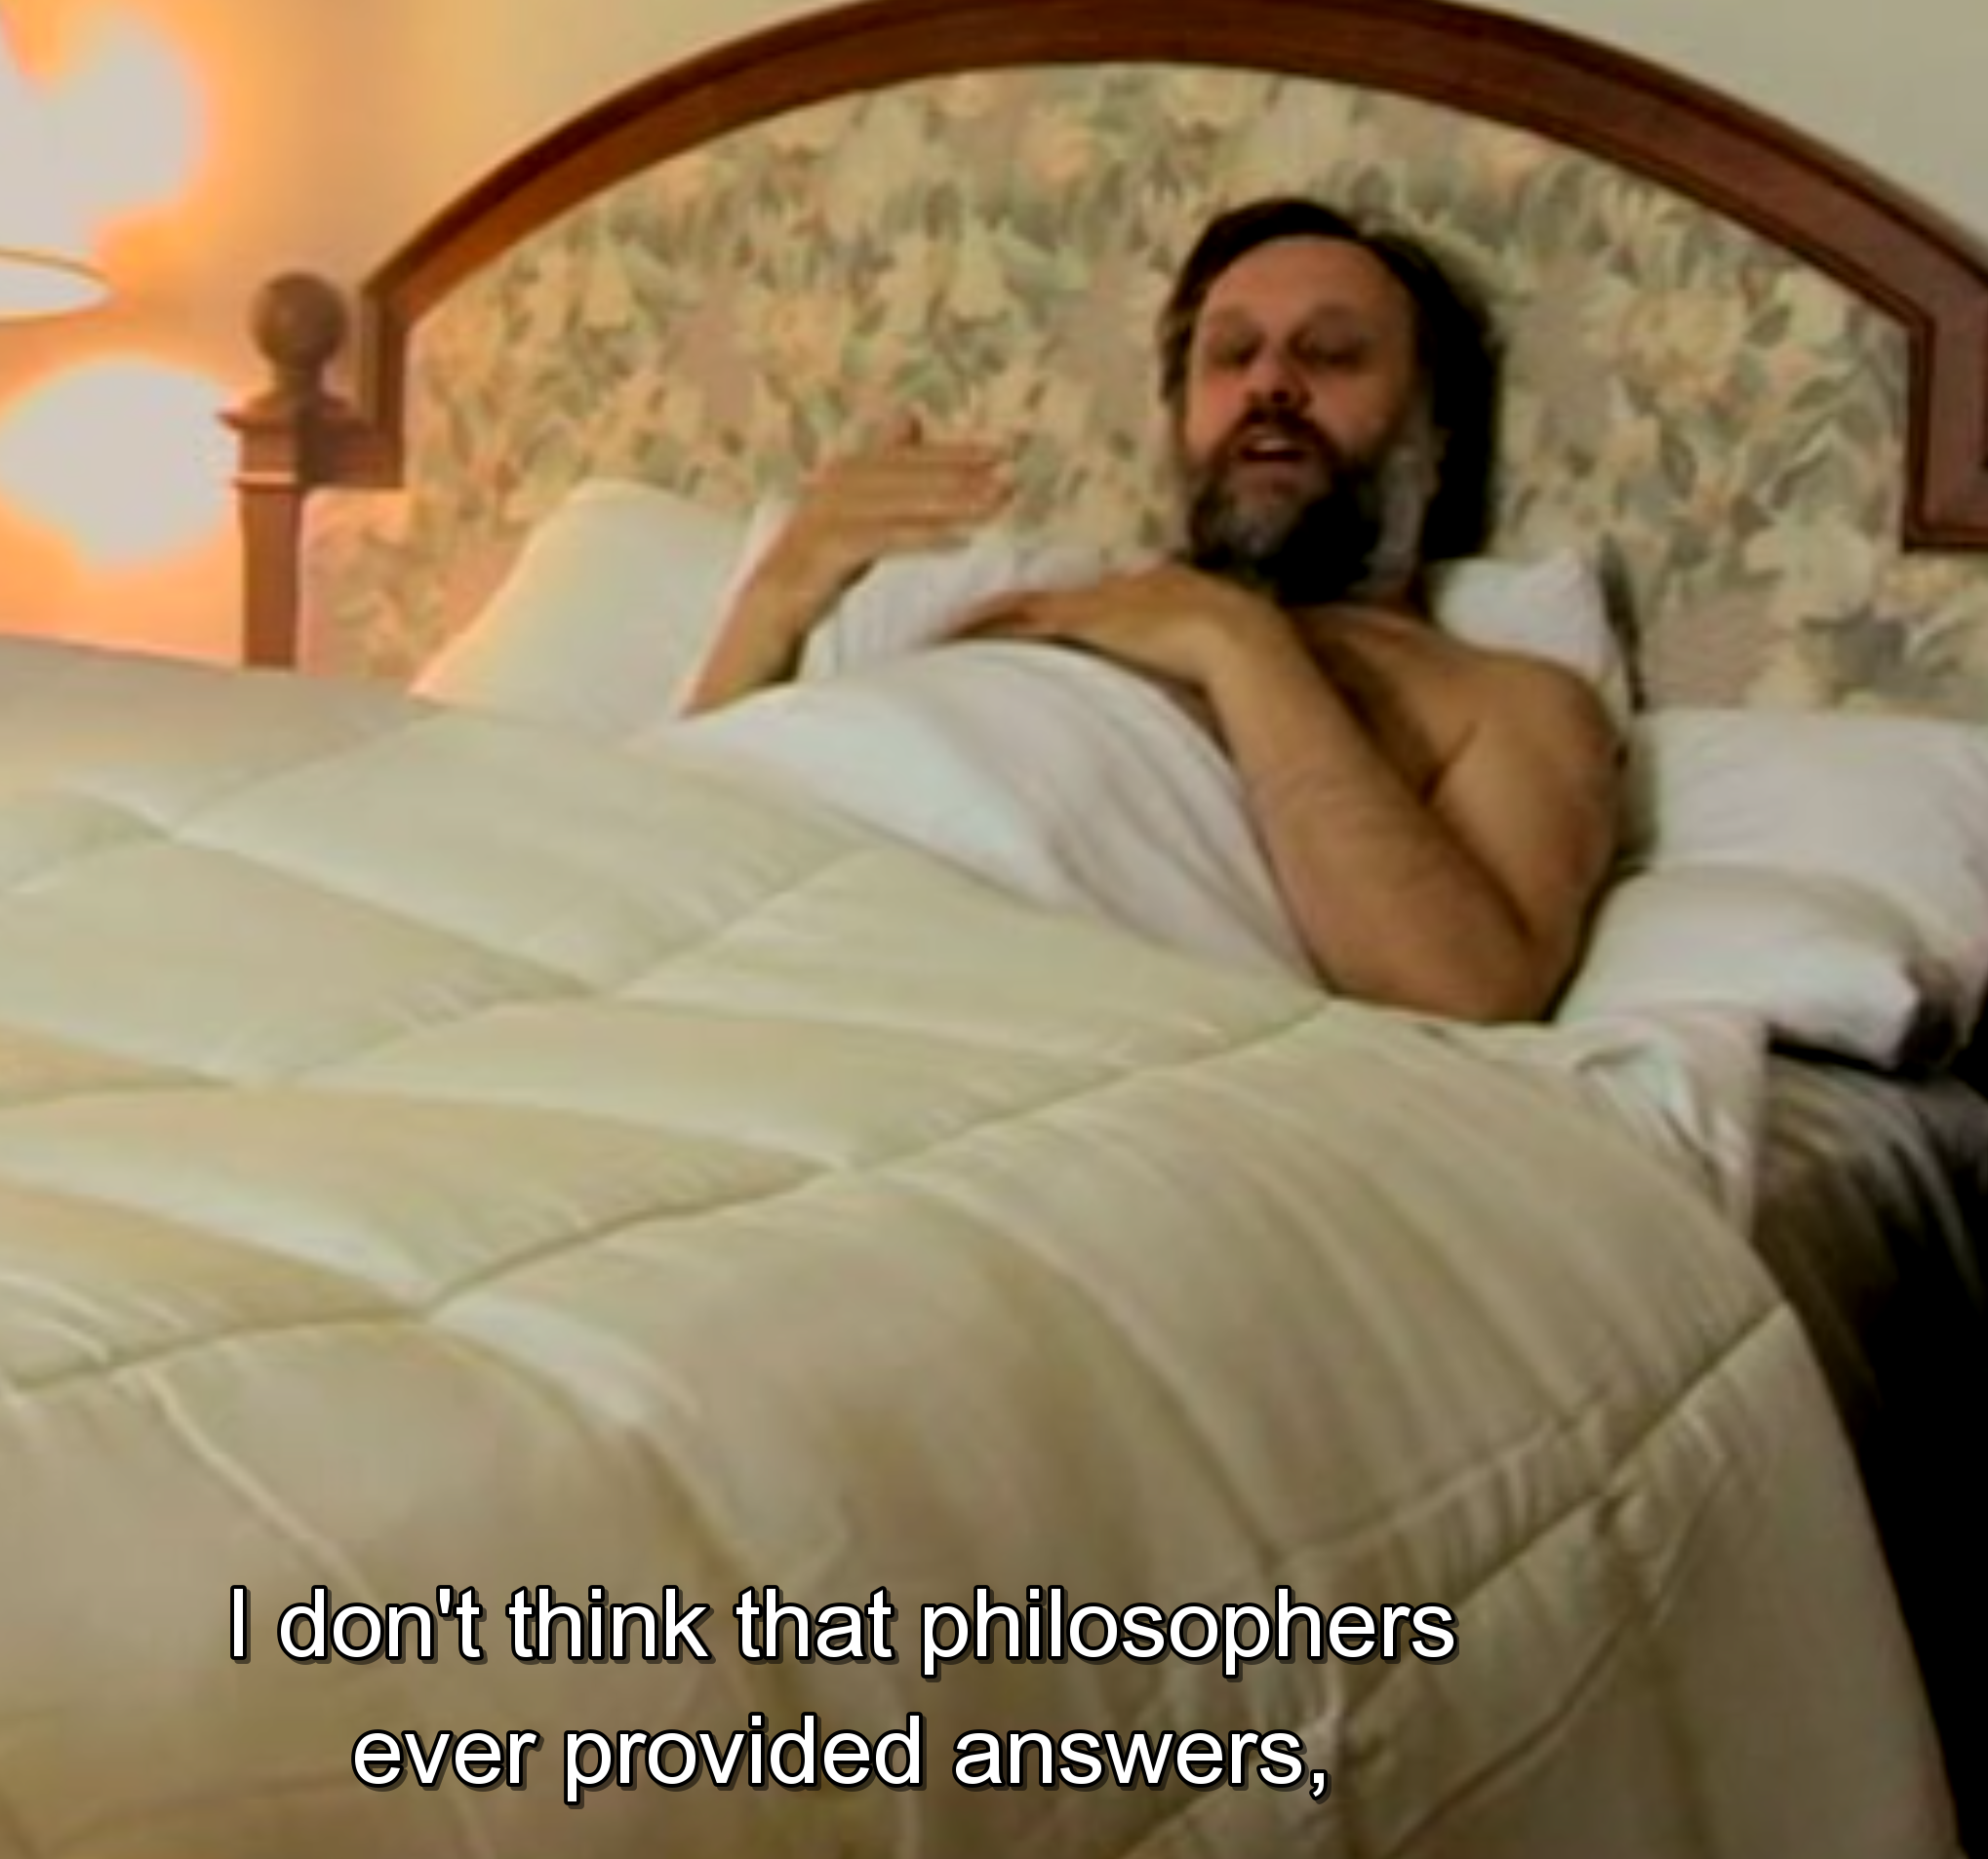
\includegraphics[width=0.5\textwidth]{images/template.png}
%	\caption{Template Bild}
%	\label{fig:template}
%\end{figure}

\end{document}
